Una significativa parte del impacto de las computadoras en los distintos aspectos de las 
ciencias e incluso de la vida diaria se debe al crecimiento de su
poder de c\'omputo desde la aparici\'on de los primeros microprocesadores hasta el
d\'ia de hoy.

Entre 1986 y 2002, la performance de los procesadores crec\'io en promedio, un 50%
por a\~no~\cite{Pacheco}, en parte gracias a la denominada \textit{Ley de Moore}, que 
establec\'ia que la densidad de transistores por circuito integrado se duplicaba 
cada 18 meses~\cite{HennessyPatterson}. Esto puede verse en la figura~\ref{processor_performance},
que compara los resultados de los \textit{benchmarks} SPEC de procesadores en distintos
momentos de la historia con respecto al procesador VAX-11/780. 

Este comportamiento consistente permiti\'o durante mucho tiempo a los desarrolladores 
de aplicaciones escribir programas de manera serial, sabiendo que al poco tiempo los procesadores
mejorar\'ian, y la performance en tiempo de ejecuci\'on de sus c\'odigos de aplicaci\''on con ellos (fen\'omeno denominado
\textit{hardware free lunch}.

\begin{figure}[htbp]
    \centering
    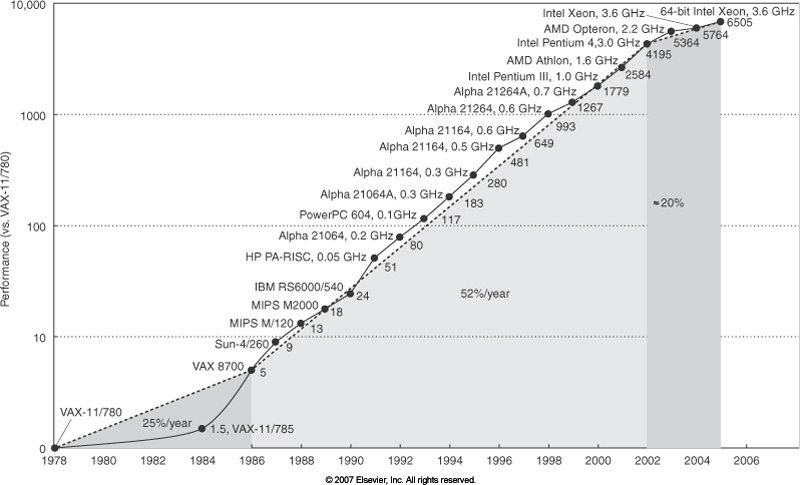
\includegraphics[width=\textwidth]{images/processor-performance.jpg}
    \caption{Performance de procesador en los \textit{benchmarks} SPEC on respecto a VAX-11/780. Tomado de~\cite{HennessyPatterson}}
    \label{processor_performance}
\end{figure}

Sin embargo, a medida que los transistores han disminuido su tama\~no, han incrementado
su disipaci\'on, limitandose entonces la cantidad que se puede ubicar de los mismos
en un circuito sin producir que el mismo se comporte de manera err\'atica producto
de la elevada temperatura de operaci\'on. El impacto de esto puede verse en que,
desde 2002, la performance de los monoprocesadores ha visto su crecimiento disminuir
a un 20\%, y en que se ha modificado el enfoque de dise\~no de procesadores, empezando
a hacerse m\'as y m\'as com\'un el uso de multiprocesadores (multiples procesadores
por chip).

El impacto en el desarrollo de aplicaciones que necesiten explotar todo el poder
de computo posible es significativa. En simulaciones para \'areas de biolog\'ia,
medicina, qu\'imica o metereolog\'ia es de invaluable utilidad mejorar los tiempos
de ejecuci\'on para permitir mejores implementaciones de los modelos utilizados,
que permiten realizar predicciones de mayor calidad. Aprovechar estas nuevas 
arquitecturas multiprocesador requiere modificaciones en el c\'odigo, a diferencia
del crecimiento en velocidad de \textit{clock} que no requer\'ia modificaciones
en el dise\~no del programa. Los intentos de escribir programas que conviertan
programas seriales (dise\~nados para un solo procesador) a paralelos, en lenguajes
de prop\'osito general como C,C++ o Fortran, han sido relativamente infructosos.

El resultado es que es necesario trabajo a nivel de escritura del \textit{software}
para utilizar multiples procesadores. La aparici\'on de nuevas herramientas ayudan
al programador en esta tarea. Un ejemplo de esto es Nvidia CUDA (\textit{Compute
Unified Device Architecture}), que provee un lenguaje de programaci\'on unificado
para el desarrollo de aplicaciones que exploten la arquitectura de unidades GPGPU
(\textit{General Purpose Graphical Processing Units}). Otros ejemplos los podemos
ver en APIs y librer\'ias unificadas de desarrollo como OpenMP o MPI 
(\textit{Message Passing Interface}), y compiladores optimizantes como Intel ICC.
Las mismas no son \textit{silver bullets}, ya que la divisi\'on de trabajo depende 
fundamentalmente del problema a resolver, en base a las dependencias entre tareas 
que tiene la soluci\'on al mismo.

En este trabajo buscaremos comparar distintas arquitecturas de hardware y como 
las caracter\'isticas espec\'ificas de la simulaci\'on qu\'imica a realizar permiten
o impiden paralelizaci\'on de trabajo en los distintos recursos que cada 
arquitectura provee.
